\documentclass[12pt]{article}

\usepackage{lastpage} % Required to determine the last page for the footer
\usepackage{extramarks} % Required for headers and footers
\usepackage{graphicx} % Required to insert images
\usepackage{listings} % Required for insertion of code
\usepackage{courier} % Required for the courier font
\usepackage{color}

% Margins
\topmargin=-0.45in
\evensidemargin=0in
\oddsidemargin=0in
\textwidth=6.5in
\textheight=9.0in
\headsep=0.25in

\linespread{1.1} % Line spacing

\vspace{4em}

\newcommand{\Title}{Software Architecture Specification Document} % Assignment title
\begin{document}

	\begin{center}%
		\LARGE \bf \Title \\[2em]
		\Large {Project:}\\
		Financial markets simulation with multiple competing algorithmic trading entities.\\[0.7em]
		\Large {Client:}
		Cortical Systems\\[2em]
		\LARGE {\bf Group:}\\
			\begin{figure}[ht!]
				\centering
				
\includegraphics[scale=0.4]{Logo8.png}
			\end{figure}
			
		\Large {\bf Members:}\\[0.3em]
		\large
		Daniel Makgonta 12147100\\
		Moeletji Semenya 12349136\\
		Madimetja Shika 12127877\\[3em]
	
	\small Publication Date: 21 May 2014\\[0.5em]
	\small Version: 0.0 		    
	\end{center}%
	
	\newpage		
	\large 
 	{\bf Change Log}\\[1em]
	\begin{tabular}{llll}
		Date & Name & Reason & Version \\
		13/05/2014 & Moeletji & Creation & 0.0 \\
		16/05/2014 & Moeletji & Adding functional requirements & 0.0 \\
		19/05/2014 & Daniel & Added Architectural Requirements & 1.0 \\
		21/05/2014 & Madimetja & Editing & 0.0
	\end{tabular}
	

	
	\newpage
	\tableofcontents
				  
	\newpage
	\section{Architectural requirements}	    
			    \subsection{Architectural scope}	

                                \begin{itemize}
                                     \item The Java programming language will be used for main processing which will include using concurrent execution of Market Participants for a realistic simulation.
                                     \item MySQL is the database that will be used for the persistent infrastructure and will record Market Data to be used for historical data as well as assisting in some strategies to perform optimally.
                                     \item All reporting functions will be use JReport(Java Report).
                                     \item Interface will be displayed using Java libraries Java�s AWT and Swings library.
                                     \item JFreeChart will be used as the API for displaying the simulation in a graphical and statistical manner. The charts will show real-time technical indicators.
                                     \item Full API of the system will be generated by Doxygen.
                                 \end{itemize}

			    \subsection{Quality requirements}	
			    	\subsubsection{Security}
			    	\begin{itemize}
			    		\item Only system administrators may tweak trading algorithms or matching engine to follow current trends within the stock market.
                                        \item The system allows anonymity in terms of no buyer or seller can view what another buyer or seller�s activities.
                                        \item Matching engine is only allowed to be accessed directly by system administrators. 
                                        \item The matching engine is abstracted to the buyers and sellers of the system. 
                                        \item System administrators are not allowed to participate in the trading simulation.
			    	\end{itemize}	
			    		
			    	\subsubsection{Auditability}
			    	\begin{itemize}
				    	\items One should be able to query any entity within the system, this includes the user who made the change, the data that was changed, the new and old values of the data, as well as when the data was changed
			    	\end{itemize}
			    	
			    	\subsubsection{Testability}
			    	\begin{itemize}
			    		\item All services provided by the system must be testable with unit tests, that that the service is provided if all pre-conditions are met (i.e. that no exception is raised except if one of the pre-conditions for the service is not met), and that all post-conditions hold true once the service has been provided. JUnitEE will be used for unit testing.
			    	\end{itemize}
			    
			    	\subsubsection{Usability}
			    	\begin{itemize}
			    		\item 100% of all registered users of the system will be able to buy and sell shares concurrently.
                                        \item The system will be presented in the English language, and with further development will cater for other popular languages.
                                        \item The Graphical User Interface will use design principals and usability goals from interaction design theoretical frameworks to increase the ease of using the system for the first time.
                                        \item All calculations will be abstracted for the users and the Graphical User Interface will only show averages and final results to the user.
                                        \item The user interface will be simplified in order to speed up the amount of trading and increase concurrency.
                                \end{itemize}
			    
			    	\subsubsection{Scalability}
			    	\begin{itemize}
			    		\item The system will be able to use multiple competing trading algorithms and allow more algorithms to be plugged in at a later stage by using inheritance, polymorphism and the Template design pattern to achieve this.
                                        \item The system will be able to concurrently trade with 20-40 Market Participants trading 1-3 different Market Entities effectively and accurately according to the business rules of the system.
                                        \item The system will be implemented using Java and will have an API that can be used with different interfaces. 
                                \end{itemize}
			    	
			    	\subsubsection{Performance}
			    	\begin{itemize}
			    		\item The matching engine will return matches in less than 1 second
                                        \item Reporting of the market will be displayed in less than 10 seconds
                                        \item The buyers and sellers will be able the concurrently interact with the market simulation and this would take less than 1 second
                                \end{itemize} 
			    	    		
                            \subsection{Access Channel Requirements}
                                 The system is a stand-alone system and does not integrate with any other systems.
                                 The system will be accessible by human users through the following channel:
                                         \begin{itemize}
                                             \item From any system that contains a JVM (Java Virtual Machine).
                                         \end{itemize}
			   			
                            \subsection{Architectural Constraints}	
                                    \begin{itemize}
                                            \item System runs on a JVM
                                            \item System uses MySQL as its database
                                            \item Operating systems: Windows, Linux, Mac OS X
                                    \end{itemize}						    	    
		\subsection{Architectural patterns/styles}
                                \begin{itemize}
                                    \item Interface segregation: system has an API that can be used by other interfaces other than its native interface.
                                    \item Singleton: the system only allows an instance of one Stock Exchange to prevent overwhelming the system�s resources. With improved system the system may be adapted to work with more than one stock exchange
                                    \item Polymorphism: All strategies inherit from a base strategy, but all sub-types have different strategies.
                                    \item Encapsulation: All Stocks are encapsulated by their managers to allow for further extensibility of the functionality.
                                \end{itemize}
                \subsection{Architectural Tactics and Strategies} 
                    \begin{itemize}
                        \item Full separate functional API allows for pluggable application interfaces.
                        \item Multi-Threading Market Participants allow for real-time simulation.
                    \end{itemize}

                \subsection{Technologies}
                    \begin{itemize}
                        \item \textbf{Software:} Java
                        \item \textbf{IDE:} Netbeans
                        \item \textbf{Database:} MySql (Database)
                        \item \textbf{Programming Languages:} Java
                        \item \textbf{Business logic:} Java
                        \item \textbf{Interface:} Java
                    \end{itemize}
			    		    		    			    	
	\section{Functional requirements and application design}
		\subsection{Introduction}	
		This part of the document outlines the functional requirements of the \textit{Financial market simulation} at the different levels of granularity. 
					    
		\subsection{Required functionality}	
				\subsubsection{Matching Engine}
				\begin{itemize}
					\item Requirement Prioritization: Critical
					\item Requirement Source: Client 	
					\item Requirement Level: High
				\end{itemize}
				This is the core of the whole system. The following functionality should be provided:
					\begin{itemize}
						\item Provide a mechanism for accepting and maintaining market depth of bids and offers.
						\item Match the different types of market orders(e.g. primarily bids and offers).
						\item Notifying the relevant market participants of the matches involved in(if any).
						\item Report market data back to market participants.
					\end{itemize}
				So all bids and offers will be dealt with by the matching engine.	
				
						\begin{figure}[th]
						\centering
						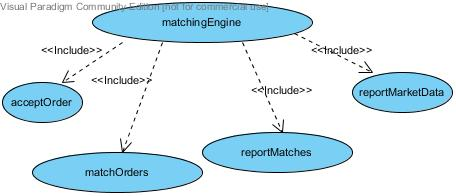
\includegraphics[scale=0.8]{./matching_engine_use_case}
						\caption{Use case for the matching engine}
						\label{matching engine use case}
						\end{figure}
				\pagebreak
				\subsubsection{Allow for multiple market participants}
				\begin{itemize}
					\item Requirement Prioritization: Critical
					\item Requirement Source: Client
					\item Requirement Level: High 	
				\end{itemize}
				Enable multiple market participants to be active in the market and allow for concurrent bids and offers to be placed. With this functionality, we can see how the market performs under certain(e.g. conditions when a stock is trending or when the market is liquid). 
				
				\subsubsection{Algorithmic trading entities}
				\begin{itemize}
					\item Requirement Prioritization: Critical
					\item Requirement Source: Client 	
					\item Requirement Level: High
				\end{itemize}
				Since there are multiple participants who will be competing in the market, we need to see how trading stategies perform in different market conditions. Each entity will need to do the following:
					\begin{itemize}
						\item Process market data and trading events from the matching engine
						\item Decide the entry or exit point into the market using data from the matching engine.
					\end{itemize}
			\pagebreak	
				\subsubsection{User Interfaces}
				\begin{itemize}
					\item Requirement Prioritization: Critical
					\item Requirement Source: Client 
					\item Requirement Level: High	
				\end{itemize}
				This requirement should provide the following user interfaces:
					\begin{itemize}
						\item  For displaying the various metrics of the performance of any selected market participant for comparing the different algorithms' performance.
						\item For showing the full market depth and matching orders by the matching engine.
					\end{itemize}

		\subsection{Domain Objects}		  
			\begin{figure}[th]
			\centering
			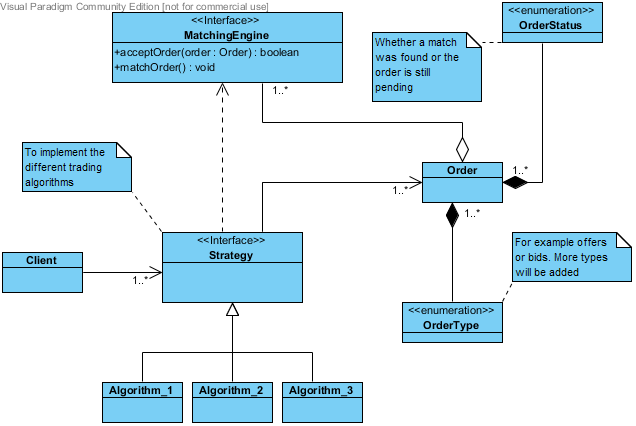
\includegraphics[scale=0.8]{./domain_objects}
			\caption{Core domain objects}
			\label{domain objects}
			\end{figure}
								
			The strategy design pattern will be used for implementing the different trading algorithms to provide pluggability.
	\newpage				
	\section{Glossary}	
		\begin{itemize}
			\item \textbf{Order}: An instruction from a participant to either put in an offer or a bid.
			\item \textbf{Market data}: Data reflecting current trading information to include pricing and volume and other additional information related to the trade.
			\item \textbf{Match}: When an offer and a bid have the same price.
		\end{itemize}				    			    			    		
\end{document}